% Source: graduate-coursework/Sp26/CSCE763/Course_Assignments/HW2/HW2_CSCE_763_solutions.tex

\documentclass[border=4pt]{standalone}
\usepackage{amsmath}
\usepackage{amssymb}
\usepackage{graphicx}
\usepackage{tikz}
\usepackage{xcolor}
\usetikzlibrary{shapes.geometric, arrows.meta, positioning, patterns, calc}

\definecolor{USC_Garnet}{HTML}{73000A}
\definecolor{USC_Sandstorm}{HTML}{FFF2E3}
\definecolor{USC_Black90}{HTML}{363636}
\definecolor{USC_Black70}{HTML}{5C5C5C}
\definecolor{USC_Black50}{HTML}{A2A2A2}
\definecolor{USC_Black10}{HTML}{ECECEC}
\definecolor{USC_Honeycomb}{HTML}{65780B}
\definecolor{USC_Atlantic}{HTML}{466A9F}
\definecolor{USC_Congaree}{HTML}{1F414D}
\definecolor{USC_Rose}{HTML}{CC2E40}
\definecolor{USC_Grass}{HTML}{CED318}
\definecolor{USC_Horseshoe}{HTML}{65780B}
\definecolor{outputbg}{RGB}{245,245,245}

\begin{document}
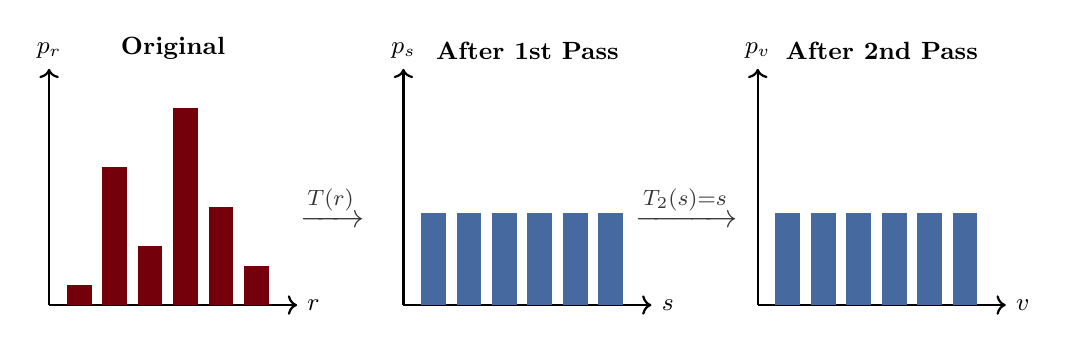
\begin{tikzpicture}[xscale=0.45, yscale=2.5]
% --- Panel 1: Original (arbitrary) ---
\begin{scope}[shift={(0,0)}]
\draw[->, thick] (0,0) -- (7,0) node[right, font=\small] {$r$};
\draw[->, thick] (0,0) -- (0,1.2) node[above, font=\small] {$p_r$};
\node[above, font=\small\bfseries] at (3.5,1.2) {Original};
\fill[USC_Garnet] (0.5,0) rectangle (1.2,0.1);
\fill[USC_Garnet] (1.5,0) rectangle (2.2,0.7);
\fill[USC_Garnet] (2.5,0) rectangle (3.2,0.3);
\fill[USC_Garnet] (3.5,0) rectangle (4.2,1.0);
\fill[USC_Garnet] (4.5,0) rectangle (5.2,0.5);
\fill[USC_Garnet] (5.5,0) rectangle (6.2,0.2);
\end{scope}
% Arrow 1
\node[font=\large, USC_Black90] at (8,0.5) {$\xrightarrow{T(r)}$};
% --- Panel 2: After 1st pass (uniform) ---
\begin{scope}[shift={(10,0)}]
\draw[->, thick] (0,0) -- (7,0) node[right, font=\small] {$s$};
\draw[->, thick] (0,0) -- (0,1.2) node[above, font=\small] {$p_s$};
\node[above, font=\small\bfseries] at (3.5,1.2) {After 1st Pass};
\foreach \x in {0.5,1.5,2.5,3.5,4.5,5.5} {
  \fill[USC_Atlantic] (\x,0) rectangle (\x+0.7,0.47);
}
\end{scope}
% Arrow 2
\node[font=\large, USC_Black90] at (18,0.5) {$\xrightarrow{T_2(s)=s}$};
% --- Panel 3: After 2nd pass (still uniform) ---
\begin{scope}[shift={(20,0)}]
\draw[->, thick] (0,0) -- (7,0) node[right, font=\small] {$v$};
\draw[->, thick] (0,0) -- (0,1.2) node[above, font=\small] {$p_v$};
\node[above, font=\small\bfseries] at (3.5,1.2) {After 2nd Pass};
\foreach \x in {0.5,1.5,2.5,3.5,4.5,5.5} {
  \fill[USC_Atlantic] (\x,0) rectangle (\x+0.7,0.47);
}
\end{scope}
\end{tikzpicture}
\end{document}
